% Drawing 146/06-4 -- folder 146, batch 06, archive page 118 (PDF page 119).
% Transcription: trois esquisses numérotées : (I) une arête $a$ terminée par une flèche, issue d'un sommet portant d'autres arêtes ; (III) une arête $a$ joignant un sommet $s$ à $s_0$, avec la mention « $s \neq s_0$ » ; (II) une boucle $a$ en $s_0$.
% Kind: local sketches of a graph at a vertex. Method 2 (schematic redraw from the facsimile). Status: ok.
% Notes: (I) an edge a ending in an arrow (a leg) at a vertex carrying other edges; (III) an edge a from s to s0, « (s != s0) »; (II) a loop a at s0. Other edges at each vertex end in dashes, as drawn.
% Coordinates: 1 unit = 1 mm = 1/100 of the crop width (bbox in page fractions: [0.07, 0.2, 0.56, 0.35]).
% Redrawn by Claude (claude-opus-5-5), issue #73 pilot, 2026-11-07; not checked by a human; not compiled (no TeX in the session).
% Rights: reproduces part of the work -- behind RENDER_TRANSCRIPTS, never published by itself.
\documentclass[tikz,border=3pt]{standalone}
\usepackage{amsmath,amssymb}
\usetikzlibrary{patterns,arrows.meta}
\tikzset{pencil/.style={black!45}, struck/.style={black!35}, mark/.style={circle,draw,inner sep=1.3pt}, pt/.style={circle,fill,inner sep=0.9pt}, opt/.style={circle,draw,fill=white,inner sep=1.1pt}}
\begin{document}
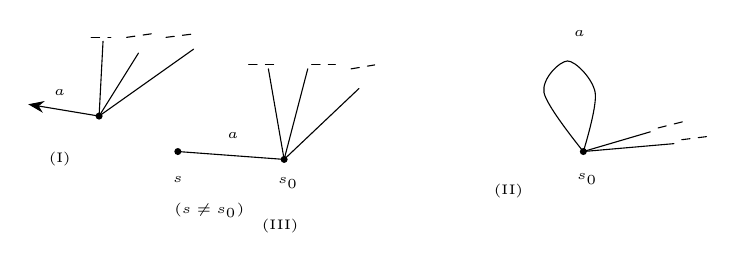
\begin{tikzpicture}[x=1mm,y=1mm,line cap=round,line join=round,font=\scriptsize]
\draw[-{Stealth[length=2mm]}] (17,-21) -- (8,-19.5);
\node[inner sep=1pt] at (12,-18) {\tiny $a$};
\draw (17,-21) -- (17.5,-11.5);
\draw (17,-21) -- (22,-13);
\draw (17,-21) -- (29,-12.5);
\node[pt] at (17,-21) {};
\draw[dashed] (16,-11) -- (18.5,-11);
\draw[dashed] (20.5,-11) -- (24,-10.5);
\draw[dashed] (25.5,-11) -- (29.5,-10.5);
\node[inner sep=1pt] at (12,-26.5) {\tiny (I)};
\draw (27,-25.5) -- (40.5,-26.5);
\node[pt] at (27,-25.5) {};
\node[pt] at (40.5,-26.5) {};
\node[inner sep=1pt] at (34,-23.5) {\tiny $a$};
\draw (40.5,-26.5) -- (38.5,-15);
\draw (40.5,-26.5) -- (43.5,-15);
\draw (40.5,-26.5) -- (50,-17.5);
\draw[dashed] (36,-14.5) -- (40,-14.5);
\draw[dashed] (44,-14.5) -- (47,-14.5);
\draw[dashed] (49,-15) -- (52,-14.5);
\node[inner sep=1pt] at (27,-29) {\tiny $s$};
\node[inner sep=1pt] at (41,-29.5) {\tiny $s_0$};
\node[inner sep=1pt] at (31,-33) {\tiny $(s\neq s_0)$};
\node[inner sep=1pt] at (40,-35) {\tiny (III)};
\draw plot[smooth, tension=0.55] coordinates {(78.5,-25.5) (73.5,-18) (76.5,-14) (80,-18) (78.5,-25.5)};
\node[inner sep=1pt] at (78,-10.5) {\tiny $a$};
\node[pt] at (78.5,-25.5) {};
\draw (78.5,-25.5) -- (87,-23);
\draw (78.5,-25.5) -- (90,-24.5);
\draw[dashed] (88,-22.5) -- (92,-21.5);
\draw[dashed] (91,-24) -- (95,-23.5);
\node[inner sep=1pt] at (79,-29) {\tiny $s_0$};
\node[inner sep=1pt] at (69,-30.5) {\tiny (II)};
\end{tikzpicture}
\end{document}
